\documentclass[letterpaper,12pt]{article}
\title{FET Inrush Protection}
\author{Chris Pavlina \\ \small \url{https://semianalog.com}}
\date{2015-11-23}

\usepackage{amsmath}
\usepackage{siunitx}
\usepackage{graphicx}
\usepackage{euler}
\usepackage{libertine}
\usepackage{float}
\usepackage{url}
\usepackage{hyperref}
\usepackage[nameinlink]{cleveref}
\usepackage{framed}
\usepackage[margin=1in]{geometry}

\newcommand{\ddt}{\ensuremath{\frac{\mathrm{d}}{\mathrm{d}t}}}
\newcommand{\dt}{\ensuremath{{\mathrm{d}t}}}

\begin{document}

\maketitle

\begin{abstract}
It is possible to use a simple one-transistor FET circuit to provide
inrush protection for low voltage DC circuits. With the addition of
only one more FET, reverse-polarity protection can also be provided.
Suggested applications include USB devices (as the USB specification
is strict about inrush) and anything requiring significant bulk
decoupling.
\end{abstract}

\begin{framed}
\textbf{TL;DR:} If you don't care how this circuit works, feel free to
skip to \cref{sec:equations} (Design equations) and \cref{sec:gotchas} (Gotchas).
\end{framed}

\tableofcontents

\section{What not to do}
\label{sec:bad}

There is a circuit that is occasionally seen\cite{elecdesign_rpp}, that adds a single capacitor
onto the familiar MOS reverse-polarity protection circuit:

\begin{figure}[H]
\centering
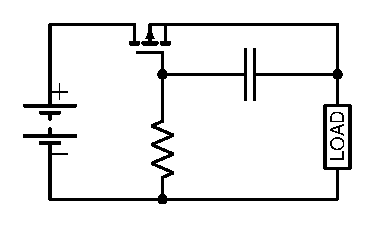
\includegraphics{what_not_to_do_1}
\caption{Don't do this!}
\end{figure}

It should be fairly obvious why this won't work. The mechanism of the reverse-polarity circuit
is that the body diode conducts until the load is \emph{almost} fully powered, and then the
voltage at the load provides enough $V_{GS}$ bias to the FET to turn it on completely. There
is nothing we can do to control the behavior of the body diode, so clearly nothing can be
built onto this circuit to slow the current.

Flipping the FET around so the body diode is no longer in circuit (losing the reverse protection
behavior) won't work either! The FET has very high voltage gain, so using an RC circuit to
ramp its gate voltage won't do much. The output voltage will still spike up quickly, allowing
a large inrush. This just \emph{delays} startup.

\section{Better, but not quite}
\label{sec:better}

What is needed is something a bit more clever:

\begin{figure}[H]
\centering
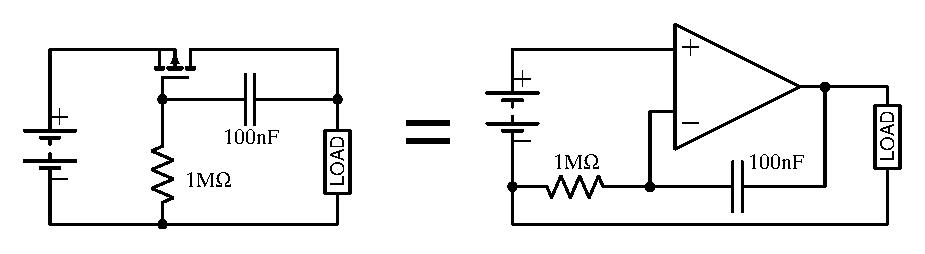
\includegraphics{what_not_to_do_2}
\caption{More clever, but still don't do it!}
\end{figure}

Imagining the FET as a differential amplifier, we can see that the circuit is actually
an integrator. When the input power is connected, the waveform seen at the input is a
step, and the integral of a step is a ramp --- perfect! If we can control the slope of
that ramp, we can easily control the inrush into our circuit's capacitance.

\section{Debugging}
\label{sec:debugging}

Let's build and test the circuit, with a \SI{12}{V} source and a
\SI{1000}{\mu F} capacitor as a load. The
inrush current of this circuit, as will be seen later in the design equations, should
be on the order of \SI{120}{mA}.

\begin{figure}[H]
\centering
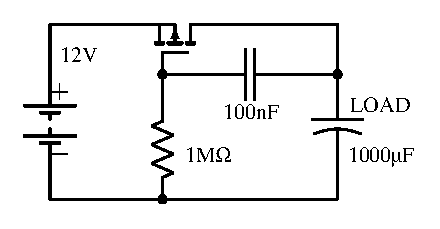
\includegraphics{what_not_to_do_3}
\caption{The circuit we're going to test.}
\end{figure}

\begin{figure}[H]
\centering
\includegraphics[width=6in]{irl_bad}
\caption{Test of faulty circuit. Channels: 1 = input, 2 = output, 3 = gate voltage, 4 = inrush current}
\end{figure}

The inrush current spikes very high, saturating the oscilloscope at well over
\SI{1.4}{A} for about \SI{1}{ms}, and sits at about \SI{200}{mA} for about
\SI{14}{ms} until it tails off.
The problem is that the FET only behaves as an integrator when it is in its
linear region of operation.  The \SI{100}{nF} timing capacitor holds the gate
to the drain as the input voltage is stepped, and the source quickly rises high
enough for this to put it in saturation.

Theoretically, any number of components can be added between the input node of
an integrator and a fixed voltage without changing the behavior of the integrator.
Taking advantage of this, we'll add a much larger capacitor between the FET's gate
and source to swamp this effect.

\section{The working circuit}
\label{sec:good}

\begin{figure}[H]
\centering
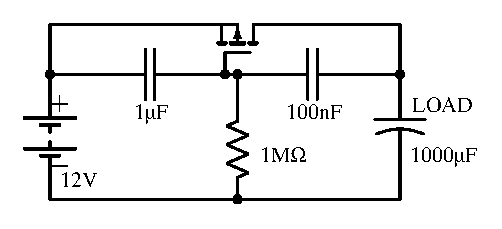
\includegraphics{do_this}
\caption{A second capacitor is added to prevent immediate saturation.}
\end{figure}

\begin{figure}[H]
\centering
\includegraphics[width=6in]{irl_plot}
\caption{Test of good circuit. Channels: 1 = input, 2 = output, 3 = gate voltage, 4 = inrush current}
\end{figure}

This one works! The additional capacitor delays startup by about \SI{250}{ms}, at which
point $V_{GS}$ reaches the threshold point and the FET begins to integrate the voltage
step. The voltage rises at about \SI{57}{V/s}, giving an inrush current of at most
about \SI{55}{mA}.

\section{Deriving the design equations}
\label{sec:deriving}

The circuit is essentially just an integrator:

\begin{figure}[H]
\centering
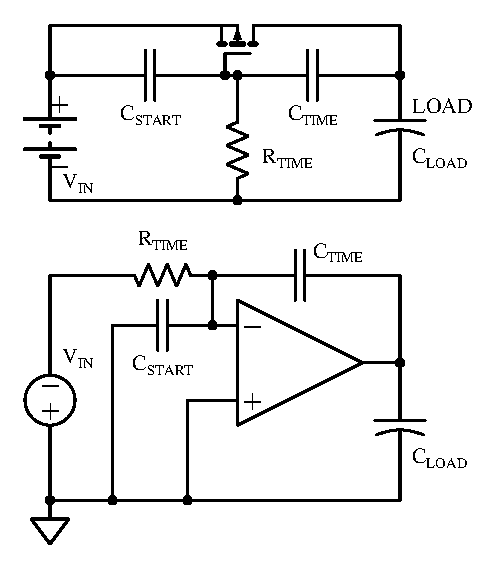
\includegraphics{ckt_labeled}
\caption{The full circuit and its equivalent integrator.}
\end{figure}

Note that the equivalent integrator circuit ``sees'' the input step as the \emph{negative}
of the input voltage. This is because the noninverting input (the FET's source) sits at the
positive rail, and the timing resistor runs to the negative rail.

The behavior of an integrator is\cite[p. 230]{aoe}:

$$ V_{out}(t) = \frac{-1}{R\cdot C} \int V_{in}(t)\;\mathrm{d}t + \mathrm{const} $$

For a stepped input voltage, we can rearrange this to get the slope of the output:

$$ \ddt V_{out}(t) = \frac{-1}{R\cdot C} V_{in}(t) $$

In the ideal integrator circuit above, the voltage across $C_{START}$ will be zero at
all times, so it can be ignored. Therefore, the slope of the output voltage will be:

$$ \ddt V_{out}(t) = \frac{V_{IN}}{R_{TIME}\cdot C_{TIME}} $$

A capacitor behaves according to $i = C \cdot \ddt v$ \cite[p. 19]{aoe}, so we can find the
current into the capacitor:

$$ I = C_{LOAD} \cdot \ddt V_{OUT} = \frac{C_{LOAD}\cdot V_{IN}}{R_{TIME}\cdot C_{TIME}} $$

The ramp time will be equal to the input voltage divided by the slope:

$$ t_{RAMP} = \frac{V_{IN}}{\ddt V_{OUT}} $$

We must compute the power dissipation in the FET to select an appropriate one. The instantaneous
power dissipation is:

$$ p(t) = (v_{out} - v_{in})\cdot i_{out} $$

The average over the pulse is:

$$ P = \frac{1}{t_{RAMP}} \int \left( (v_{out} - v_{in}) \cdot i_{out} \right) \dt $$

$i_{out}$ is constant, and $v_{out} - v_{in}$ is a linear slope, making the area under this curve
triangular. The integral can be computed geometrically:

$$ A_{triangle} = \frac{1}{2} (w \cdot h) $$

$$ P = \frac{1}{t_{RAMP}} \cdot \frac{1}{2} \left( V_{IN} \cdot t_{RAMP} \cdot I_{OUT} \right) $$

$$ P = \frac{1}{2} \left( V_{IN} \cdot I_{OUT} \right) $$

Now, we must derive $C_{START}$. At inrush, $C_{START}$ and $C_{TIME}$ behave as a capacitive
voltage divider, and these must keep $V_{GS}$ between zero and the threshold voltage at all
times.

$$ V_{GS} = V_{IN} \cdot \frac{C_{TIME}}{C_{TIME} + C_{START}} $$

$$ C_{START} = C_{TIME} \cdot \left( \frac{V_{IN}}{V_{GS(th)}} - 1 \right) $$

This equation describes the critical case, so for error margin we want:

$$ C_{START} > C_{TIME} \cdot \left( \frac{V_{IN}}{V_{GS(th)}} - 1 \right) $$

\section{Design equations}
\label{sec:equations}

\begin{figure}[H]
\centering
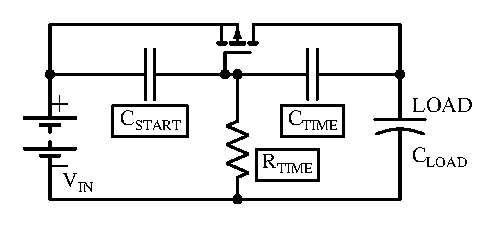
\includegraphics{just_ckt_labeled}
\caption{The full circuit with parts labeled. Unknowns are in boxes.}
\end{figure}

\begin{enumerate}
\item{The input voltage $V_{IN}$ and the load capacitance $C_{LOAD}$ are known as part
    of your application.}
\item{Determine $I_{INR}$, the desired inrush current.}
\item{Compute the resulting output voltage slope, $\ddt V_{OUT}$:

    $$ \ddt V_{OUT} = \frac{I_{INR}}{C_{LOAD}} $$ }
\item{Select $R_{TIME}$ and $C_{TIME}$. Note that either one of them can be freely chosen,
    and the other one computed:

    $$ R_{TIME} \cdot C_{TIME} = \frac{V_{IN}}{\ddt V_{OUT}} $$ }
\item{Compute the power dissipation and ramp time:

    $$ P = \frac{1}{2}\left( V_{IN} I_{IN} \right) $$
    $$ t_{RAMP} = \frac{V_{IN}}{\ddt V_{OUT}} = R_{TIME} \cdot C_{TIME} $$ }
\item{Select a MOSFET. Ensure that its $V_{DS}$ rating can handle the supply voltage,
its $R_{DS(on)}$ is low enough for your application, and that its FBSOA (forward-bias safe
operating area) allows for a pulse of the above computed amplitude and duration. Note its
minimum $V_{GS(th)}$ for the next part.}

\item{Compute $C_{START}$. For error margin, it should be at least double the computed
value, but do not make it \emph{too} big, or the startup delay will be unnecessarily long:

    $$ C_{START} > C_{TIME} \cdot \left( \frac{V_{IN}}{V_{GS(th)}} \right) $$}

\end{enumerate}

\section{Gotchas}
\label{sec:gotchas}

This circuit isn't perfect. There are few traps and drawbacks:

\begin{itemize}
\item{As presented, the MOSFET must have a $V_{GS(max)}$ rating in excess of $V_{IN}$.
If this is impractical, a second resistor $R_{LIMIT}$ can be placed in parallel with $C_{START}$,
forming a voltage divider to set the final gate voltage.

Perhaps counter-intuitively, this does not change the timing resistance to be the
Th\'evenin equivalent of $R_{LIMIT}$ and $R_{TIME}$, for the same reason that $C_{START}$ does
not affect the timing.}

\item{This circuit only limits capacitive inrush. If your inrush is for other reasons,
for instance $V_{DD}$ ramp inrush of a large digital device like an FPGA, it may actually
worsen it. Mind the maximum ramp times of the devices you are powering. If you have voltage
regulators downstream, it may be desirable to add an RC delay to their enable inputs to start
them after this circuit has stabilized.}

\item{This is not a precision circuit! For the example above, $I_{INR}$ should have been
$\frac{C_{LOAD} \cdot V_{IN}}{R_{TIME} \cdot C_{TIME}} = \frac{\SI{1000}{\mu F} \cdot \SI{12}{V}}{\SI{1}{M\Omega} \cdot \SI{100}{nF}} = \SI{120}{mA} $,
but it was actually \SI{55}{mA}, a massive $-54\%$ error! Note that SPICE simulation verifies the
accuracy of these equations, so other real-world effects were at play here. When using more ideal
components (accurate ceramic capacitors with low $C(V)$ dependence, in particular), the real measurements
will be closer to the predicted values.}

\item{This circuit does not provide reverse-polarity protection. It can be modified with one
additional FET, though --- dual MOSFETs with both devices in the same package are handy here:}
\end{itemize}

\begin{figure}[H]
\centering
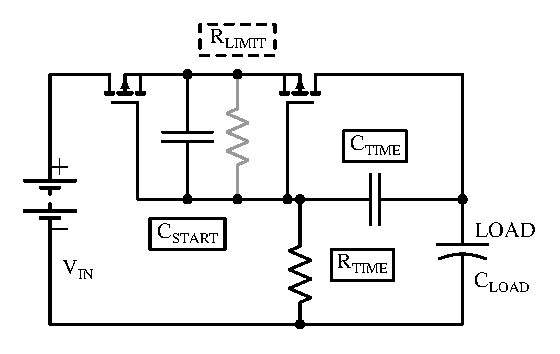
\includegraphics{with_rpp}
\caption{The full circuit with additional RPP.}
\end{figure}

\section{Worked example}
\label{sec:example}

As an example, we'll design an inrush limiter for a USB device. Specifications are:

\begin{itemize}
\item{$V_{IN}$: \SI{5}{V} nominal}
\item{$C_{LOAD}$: \SI{220}{\mu F}}
\item{$I_{OUT}$ at startup: \SI{20}{mA}}
\item{Maximum $I_{IN}$: \SI{113}{mA} \cite{usb2}}
\item{$C_{IN}$: min. \SI{1}{\mu F}, max. \SI{10}{\mu F} \cite{usb2}}
\end{itemize}

\hrulefill

\begin{enumerate}
\item{The input voltage $V_{IN}$ and the load capacitance $C_{LOAD}$ are known as part
    of the application.}
\item{$I_{IN}$ must not exceed \SI{113}{mA}, and the load will draw $I_{OUT} = \SI{20}{mA}$
    at startup, so $I_{INR}$ must not exceed $\SI{113}{mA} - \SI{20}{mA} = \boxed{\SI{93}{mA}}$.}
\item{Compute the resulting output voltage slope, $\ddt V_{OUT}$:

    $$ \ddt V_{OUT} = \frac{I_{INR}}{C_{LOAD}} $$
    $$ \ddt V_{OUT} = \frac{\SI{93}{mA}}{\SI{220}{\mu F}} = \boxed{\SI{423}{V/s}} $$ }
\item{Select $R_{TIME}$ and $C_{TIME}$. It is likely that the system will already contain
    \SI{100}{nF} capacitors, so we'll set $C_{TIME} = \boxed{\SI{100}{nF}}$.

    $$ R_{TIME} \cdot C_{TIME} = \frac{V_{IN}}{\ddt V_{OUT}} $$
    $$ R_{TIME} = \frac{V_{IN}}{C_{TIME} \cdot \ddt V_{OUT}} = \SI{118}{k\Omega} \approx \boxed{\SI{120}{k\Omega}} $$ }
\item{Compute the power dissipation and ramp time. Note that this uses $I_{IN}$, the total input
    current, not $I_{INR}$, the inrush current to the capacitor.

    $$ P = \frac{1}{2}\left( V_{IN} I_{IN} \right) $$
    $$ P = \frac{1}{2}\left( \SI{5}{V} \cdot \SI{113}{mA} \right) = \boxed{\SI{283}{mW}} $$

    $$ t_{RAMP} = \frac{V_{IN}}{\ddt V_{OUT}} = R_{TIME} \cdot C_{TIME} $$
    $$ t_{RAMP} = (\SI{120}{k\Omega})\cdot(\SI{100}{nF}) = \boxed{\SI{12}{ms}} $$ }
\item{Select a MOSFET. I'm going to use International Rectifier's IRLML6402, which has
    a low $R_{DS(on)}$ of \SI{65}{m\Omega}, a minimum $V_{GS(th)}$ of \SI{400}{mV},
    and fits the above power dissipation nicely into its FBSOA\cite{irlml6402}.}
\item{Compute $C_{START}$. For error margin, it should be at least double the computed
value, but do not make it \emph{too} big, or the startup delay will be unnecessarily long:

    $$ C_{START} > C_{TIME} \cdot \left( \frac{V_{IN}}{V_{GS(th)}} \right) $$
    $$ C_{START} > (\SI{100}{nF}) \cdot \left( \frac{\SI{5}{V}}{\SI{0.4}{V}} \right) $$
    $$ C_{START} > \boxed{\SI{1.25}{\mu F}} $$

A \SI{2.2}{\mu F} capacitor would be reasonable for $C_{START}$ and give some error margin.}

\item{The USB example is unique in that it has a \emph{minimum} input capacitance, of \SI{1}{\mu F}.
    The input capacitance of this circuit itself is the series combination of $C_{START}$, $C_{TIME}$,
    and $C_{LOAD}$, which is \SI{96}{nF}. We'll add a second \SI{2.2}{\mu F} at the input, which places
    the total input capacitance at about \SI{2.3}{\mu F}.}

\end{enumerate}

\begin{figure}[H]
\centering
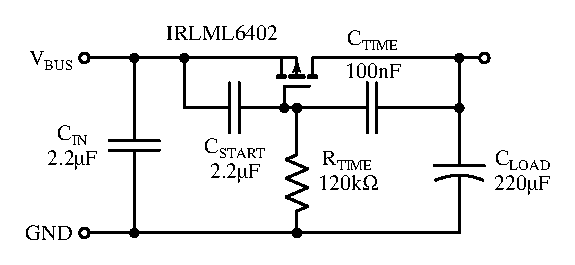
\includegraphics{worked_example}
\caption{Example with values}
\end{figure}

\begin{figure}[H]
\centering
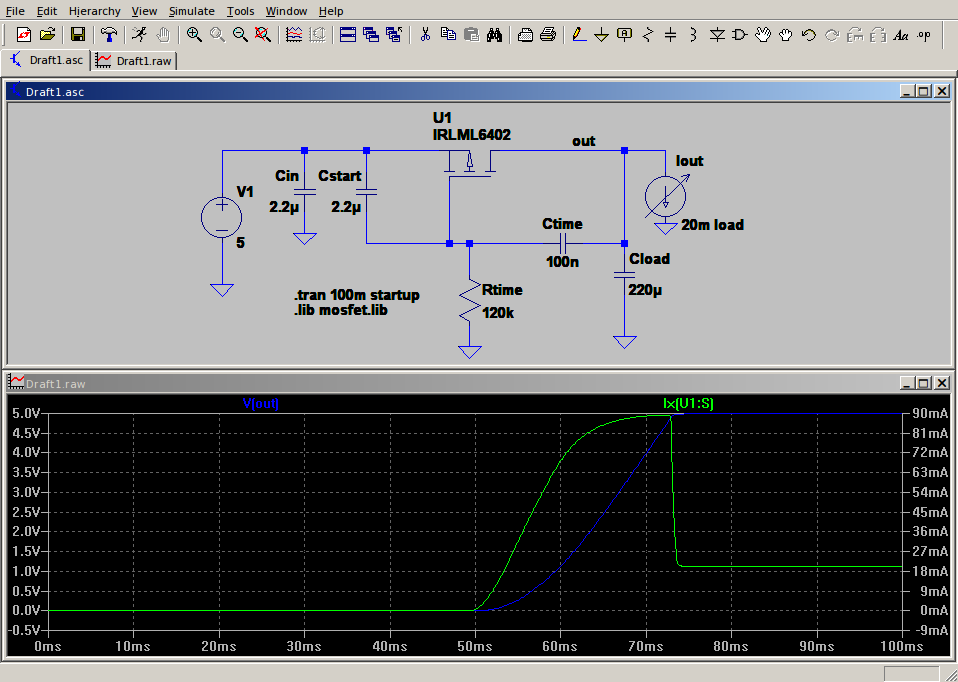
\includegraphics[width=6in]{example_sim}
\caption{Simulated example}
\end{figure}

\begin{thebibliography}{10}
\bibitem{aoe}
P. Horowitz and W. Hill, The art of electronics, 3rd ed. Cambridge [England]: Cambridge University Press, 2014.

\bibitem{irlml6402}
International Rectifier, IRLML6402PbF HEXFET\textsuperscript{\textregistered} Power MOSFET, 2014. [Online].
Available: \url{http://www.irf.com/product-info/datasheets/data/irlml6402pbf.pdf}. [Accessed: 23 Nov 2015].

\bibitem{usb2}
USB Implementers Forum, Universal Serial Bus Specification, rev 2.0. 2000, pp. 7.2.4.1. Available: \url{http://www.usb.org/developers/docs/usb20_docs/}.

\bibitem{elecdesign_rpp}
J. Walker, `FET Supplies Low-Voltage Reverse-Polarity Protection', ElectronicDesign.com, 2005. [Online].
Available: \url{http://electronicdesign.com/power/fet-supplies-low-voltage-reverse-polarity-protection}. [Accessed: 23 Nov 2015].

\end{thebibliography}

\end{document}
